\documentclass[12pt,a4paper]{article}
\usepackage[utf8]{inputenc}
\usepackage[english]{babel}
\usepackage{xstring}
\usepackage{siunitx}
\usepackage{amsmath}
\usepackage{graphicx}
\usepackage[nottoc]{tocbibind} %Adds "References" to the table of contents
\usepackage{hyperref}
\usepackage[toc]{glossaries}
\usepackage{textcomp}
\usepackage{csvsimple}
\usepackage{pgfplotstable}
\pgfplotsset{compat=1.9}% supress warning
\usepackage{longtable}
\usepackage{xcolor,colortbl}
\usepackage{listings}
\usepackage[toc,page]{appendix}
\usepackage{fancyvrb}
\usepackage{tikz}


\lstset{ %
language=C++,           % choose the language of the code
numbers=left,           % where to put the line-numbers
numberstyle=\tiny,      % the size of the fonts that are used for the line-numbers
basicstyle=\footnotesize    % the size of the fonts that are used for the line-numbers
}

\newcommand{\mc}[2]{\multicolumn{#1}{c}{#2}}
\definecolor{Gray}{gray}{0.85}
\definecolor{LightCyan}{rgb}{0.88,1,1}

\newcolumntype{A}{>{\columncolor{Gray}}c}
\newcolumntype{B}{>{\columncolor{white}}c}

% MODIFY NUMBERING OF TABLES AND PICTURES
\usepackage{chngcntr}
\counterwithin{table}{section}
\counterwithin{figure}{section}
\counterwithin{equation}{section}
\usepackage{floatrow}
\floatsetup[table]{capposition=top}

% HEADINGS AND MARGINS 
\usepackage{geometry}
 \geometry{
 a4paper,
 left=25mm,
 right=25mm,
 top=25mm,
 bottom=25mm,
 headheight=15mm,
 footskip=15mm,
 }
 

% PAGE STYLE SECTION
\usepackage{fancyhdr}
\pagestyle{fancy}
\renewcommand\sectionmark[1]{\markboth{\thesection\ #1}{}}
\fancyhf{}
\fancyhead[C]{\bfseries\leftmark}
\fancyfoot[C]{\bfseries\thepage}
\renewcommand{\headrulewidth}{0.5pt}% suppress the header rule

% INDENTATATIONS
\usepackage{indentfirst}
\setlength{\parindent}{0.75cm}

% FONT
\usepackage{times}

% UNIVERISTY LOGO TRIGGER
\usepackage{graphicx}

% TITLES OF PARTICULAR SECTIONS
\usepackage{titlesec}

\titleformat{\section}
    {\large\bfseries\itshape}
    {\thesection}
    {1em}
    {\MakeUppercase}
\titleformat{\subsection}
    {\large\bfseries\itshape}
    {\thesubsection}
    {1em}
    {}
\titleformat{\subsubsection}
    {\large\bfseries\itshape}
    {\thesubsubsection}
    {1em}
    {}
\titleformat{\paragraph}
    {\large\bfseries}
    {\theparagraph}
    {1em}
    {}
\titleformat{\subparagraph}
    {\large\bfseries}
    {\thesubparagraph}
    {1em}
    {}

\begin{document}

\begin{titlepage}
    \centering
    
\includegraphics[width=7cm]{logo.jpg} % also works with 
    \vskip1cm
    {\Large
        SILESIAN UNIVERSITY OF TECHNOLOGY\\
        FACULTY OF ELECTRICAL ENGINEERING\\
        \vskip0.5cm
        Department of Power Electronics, Electrical Drives and Robotics\\
    }
    \vskip1cm
    {\bfseries\huge
    Master's thesis\\
    }
    \vskip1cm
    {\bfseries\large
    To be determined \\
    }
    \vskip2cm
    {\large
    \begin{tabular}{p{4cm} p{10cm}}
    Student: & {\bfseries\Large Igor Aleksander JANKIEWICZ}\\
    Transcript no.: & 285947\\
        &   \\
    Type of studies: & Extramural studies (MSc programme)\\
    Field of study: & Electrical Engineering\\
    Programme: & To be determined\\
        &   \\
    Supervisor: & PhD. EEng. Andrzej Latko\\
    \end{tabular}
    }
    \vskip2.5cm
    {\large
    Gliwice 2020}
\end{titlepage}
\newpage\null\thispagestyle{empty}\newpage
\tableofcontents
\newpage\null\thispagestyle{empty}\newpage

\section{What is Energy Harvesting?}
Energy Harvesting is a process of using ambient energy by converting it into a usable form, i.e. electricity or heat. It is important to point out that energy harvesting has been around for quite a long time, since solar panels, wind turbines and water turbines are in constant use for a few decades, providing people with environmentally clean energy \cite{EnHv1}.
\vskip 5mm
There are some important issues related to any energy source that could be potentially used for harvesting. First of all, it is crucial to evaluate intensity and availability of that source. Subsequently, one should find out a cost-effectiveness of the solution as well as the influence of the harvesting process on the primary energy source \cite{EnHv1}.\par
\vskip 5mm
Vibration-based Energy Harvesting incorporates a number of different fields of study, i.e. material science, mechanics or electrical engineering, just to name a few. Last sentence implies that the analysis of a piezoelectric generator itself is not a straightforward process. The electromechanical response of this device relies thoroughly on the source of ambient energy \cite{EnHv2}.\par

\begin{figure}[h!]
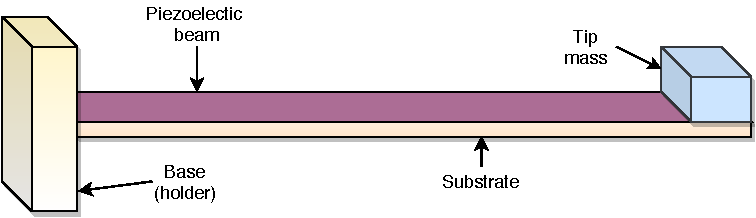
\includegraphics[scale=1]{beam1.pdf}
\end{figure}

\begin{table}[ht]
\small
\begin{center} 
\begin{tabular}{|c|c|c|c|l|}
\hline 
\textbf{Type} & \textbf{Conditions} & \textbf{Power Density} & \textbf{Area or Volume} & \textbf{Energy/Day} \\ 
\hline 
\hline
Vibration & $1m/s^2$ & $100\mu W/cm^3$ & $1cm^2$ & $8.64J$ (continuous vibration) \\ 
\hline 
Solar & Outdoors & $7500\mu W/cm^2$ & $1cm^2$ & $324J$ (sunny half a day) \\ 
\hline 
Solar & Indoors & $100\mu W/cm^2$ & $1cm^2$ & $4.32J$ (sunny half a day) \\ 
\hline 
Thermal & $\Delta T = 5 ^{\circ} C$ & $60\mu W/cm^2$ & $1cm^2$ & $2.59J$ (heat available for half a day) \\ 
\hline 
\end{tabular} 
\end{center}
\caption{Common data for some of Energy Harvesting Sources \cite{EnHv1}}
\label{tab:typdat}
\end{table}

\section{Measurement setup design}

A proper measurement process is a crucial part of this project. Having said that, a custom data acquisition board is to be designed.
\par

First of all, it is vital to highlight most important features required to achieve desired performance. There are four major aspects that have to be taken into account, namely, the ADC resolution as well as the input voltage range, the bandwidth and high input impedance of the analog front-end. Apart from that, one should take care of easy interfacing to personal computer, thus compact size and USB interface would be considered as huge assets.
\par
The previous paragraph introduced briefly main functionalities of the target device. It is quite easy to notice that there would be a lot of trade-offs to consider through the design process. Compact size and the complex analog circuitry usually do not mix, especially when planning to get a device of USB mass storage size. These facts are forcing the designer to look for a microcontroller that provides decent ADCs, also in terms of the sampling rate. Since the project is dealing with piezoelectric generators, there is always a risk of relatively high voltages at the input terminals, especially when harvesters are not connected to any load. To face this problem, the data acquisition board would be equipped with two different means of protection. The first one takes care of the input stage of the device. The second one is a classic galvanic isolation between the microcontroller (as well as the analog front end) and the personal computer. This way, there is no risk of damaging host devices utilizing the data acquisition system. The summary of the above-mentioned description is presented in the Figure~\ref{fig:meas_overview}.\par

\begin{figure}[h!]
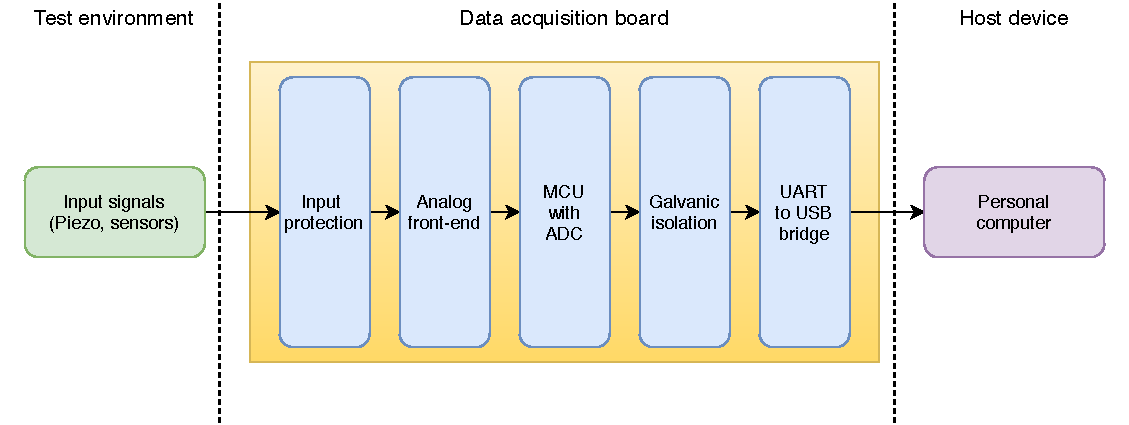
\includegraphics[scale=0.8]{measurement_setup_overview.pdf}
\caption{Measurement setup overview}
\label{fig:meas_overview}
\end{figure}

\subsection{Design requirements}
The first step of the design process is to determine desired input ratings as well as data acquisition capabilities. The piezoelectric device used in this project would be the major signal source during all experiments. Its datasheet \cite{PPA} does not state the exact any fixed maximum ratings. Instead, it provides exemplary results obtained by varying acceleration amplitude, frequency, tip mass and load resistance - see Table \ref{tab:ppapower}.\par

\begin{table}[ht!]
\centering
\begin{tabular}{|c|c|c|c|c|c|c|}
\hline
\multicolumn{1}{|c|}{\textbf{\begin{tabular}[c]{@{}c@{}}Acceler.\\ ampl. $(g)$\end{tabular}}} & \multicolumn{1}{c|}{\textbf{\begin{tabular}[c]{@{}c@{}}Freq.\\ $(Hz)$\end{tabular}}} & \multicolumn{1}{c|}{\textbf{\begin{tabular}[c]{@{}c@{}}Tip mass\\ $(gram)$\end{tabular}}} & \multicolumn{1}{c|}{\textbf{\begin{tabular}[c]{@{}c@{}}RMS\\ power $(mW)$\end{tabular}}} & \multicolumn{1}{c|}{\textbf{\begin{tabular}[c]{@{}c@{}}RMS\\ voltage $(V)$\end{tabular}}} & \multicolumn{1}{c|}{\textbf{\begin{tabular}[c]{@{}c@{}}RMS\\ current $(mA)$\end{tabular}}} & \textbf{\begin{tabular}[c]{@{}c@{}}Load\\ $(k\Omega)$\end{tabular}} \\ \hline
0.25                                                                                                 & 132                                                                                    & 0.0                                                                                     & 0.1                                                                                    & 1.1                                                                                     & 0.1                                                                                      & 17.9                                                                 \\
0.50                                                                                                 & 131                                                                                    & 0.0                                                                                     & 0.2                                                                                    & 1.9                                                                                     & 0.1                                                                                      & 18.3                                                                 \\
1.00                                                                                                 & 131                                                                                    & 0.0                                                                                     & 0.7                                                                                    & 3.4                                                                                     & 0.2                                                                                      & 15.7                                                                 \\
2.00                                                                                                 & 129                                                                                    & 0.0                                                                                     & 2.2                                                                                    & 5.4                                                                                     & 0.4                                                                                      & 13.0                                                                 \\ \hline
0.25                                                                                                 & 60                                                                                     & 1.9                                                                                     & 0.1                                                                                    & 2.9                                                                                     & 0.0                                                                                      & 61.0                                                                 \\
0.50                                                                                                 & 60                                                                                     & 1.8                                                                                     & 0.5                                                                                    & 3.3                                                                                     & 0.2                                                                                      & 20.8                                                                 \\
1.00                                                                                                 & 60                                                                                     & 1.7                                                                                     & 1.8                                                                                    & 7.1                                                                                     & 0.3                                                                                      & 28.6                                                                 \\ \hline
0.25                                                                                                 & 22                                                                                     & 22.8                                                                                    & 1.4                                                                                    & 9.0                                                                                     & 0.1                                                                                      & 60.4                                                                 \\
0.50                                                                                                 & 22                                                                                     & 22.8                                                                                    & 4.4                                                                                    & 17.3                                                                                    & 0.3                                                                                      & 67.6                                                                 \\ \hline

\end{tabular}
\caption{Exemplary piezoelectric harvester response. Data from PPA-1001 datasheet \cite{PPA}}
\label{tab:ppapower}
\end{table}

As mentioned in the previous paragraph, there is no constrained area in terms of vibration frequency and level stated by the manufacturer. Based on the data presented in the Table \ref{tab:ppapower}, the designer is relatively free to determine the operating frequency range as well as the expected input signal captured at the harvester output. When considering bandwidth and sampling rate, it is important to take into account the Nyquist criterion. It states that the sampling rate has to be twice the highest frequency in the signal \cite{ElEx}. Assuming maximum vibration frequency of 500Hz, more than 1000 samples per second need to be captured.
\par

Of course, this sampling rate only allows to reproduce an incoming signal (sinusoidal wave) as a corrupted triangle, since there is not enough data points to accurately reflect the sine shape. To solve this problem, the sampling rate should be increased by factor of 5 or so, what ultimately yields at least 5000 samples per second (sps). To illustrate the problem, Figure \ref{fig:nyquist} is introduced. It can be easily seen that sampling rate as high as twice the input signal frequency is definitely not enough. Having said that, the minimum expected sampling rate is to be at least 5000 sps.
\par

\begin{figure}[h!]
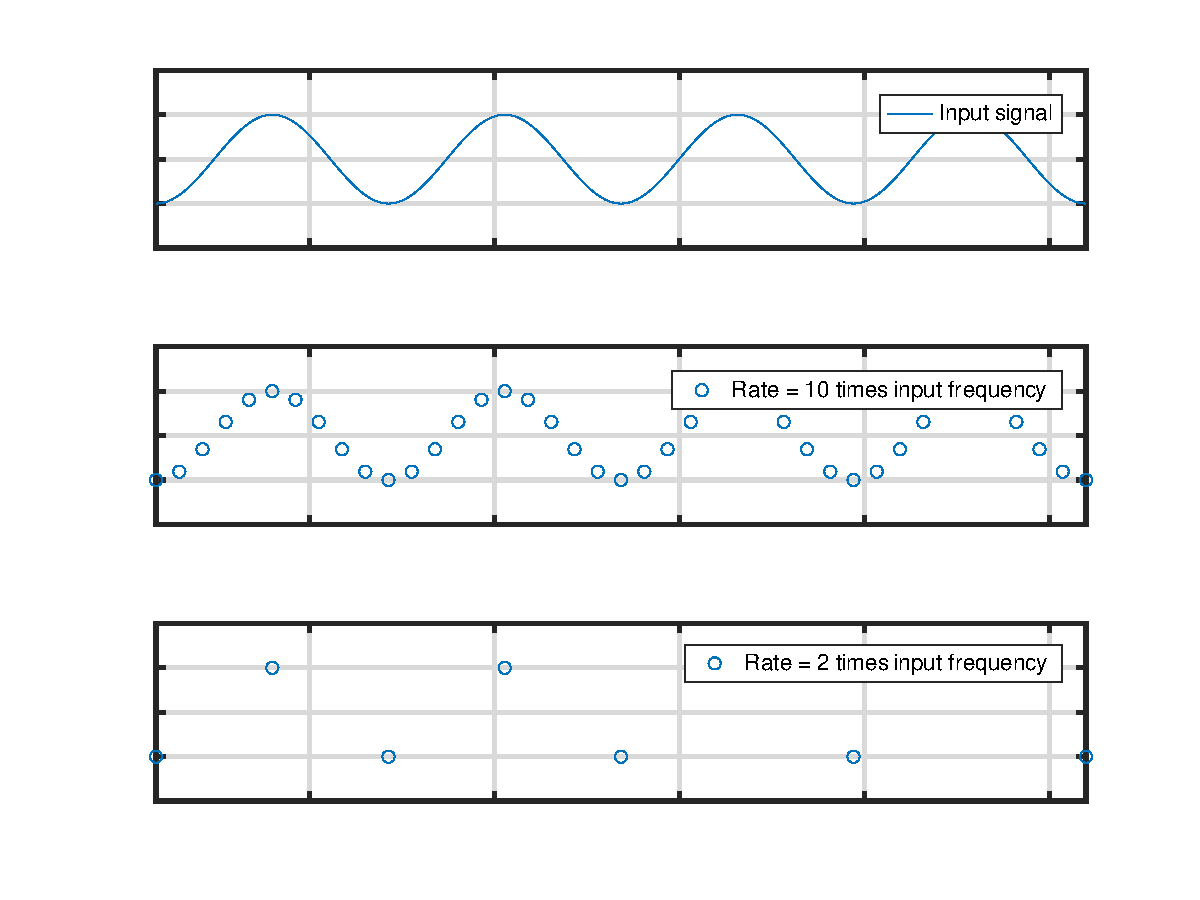
\includegraphics[scale=0.75]{nyquist.pdf}
\caption{Captured waveform versus sampling rate}
\label{fig:nyquist}
\end{figure}

It is likely that the microcontroller used in the data logger would use some kind of a serial communication protocol. Assuming that more than one signal is recorded at the time and the baud rate is fixed at the same level, the maximum input signal frequency would be divided by the number of active channels. For example, for 2 channel measurement, the maximum input signal frequency is 250Hz and so on.
\par

One of the previous paragraphs mentioned the piezoelectric harvester as the main input signal source. Knowing that the device produces a sinusoidal output, the analog front-end has to be able to capture AC signals, preferably of a relatively high amplitude. This requirements force the designer to develop symmetrical power supply for the input section as well as the circuitry allowing to add offset to the signal before it reaches the ADC input. A reason is that the ADC of the microcontroller is likely to accept only unipolar signals within tightly specified range. Remaining channels would be able to interface DC signals only, what makes them suitable for external sensors such as the accelerometer.
\par

When considering the maximum input signal level, one has to note that it should not exceed supply voltage of operational amplifier used in the input section. In case of the designed device, the power supply would be industrial $+/-$15VDC, as it would help to maintain compatibility with wide range of available operational amplifiers. Based on the last sentence, the maximum input voltage is specified to $+/-$15V for the AC input and $+$15V for DC inputs. In order to assure proper operating conditions for the analog-front end, an additional input protection is to be provided.
+
\newpage

\bibliography{bibliography} 
\bibliographystyle{ieeetr}

\end{document}
